\hspace*{-1.2cm} 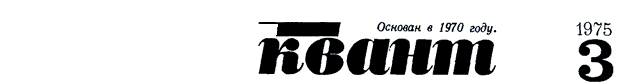
\includegraphics{lt1}
\vspace*{-1cm}
\begin{wrapfigure}[8]{l}{0.64\textwidth}
\hspace*{-0.4cm}
\includegraphics[width=0.68\textwidth]{lt2}
\end{wrapfigure}

\begin{spacing}{0.7}
\vspace*{0.1cm}
\noindent\textit{Научно-популярный\\
физико-математический\\
журнал\\
Академии наук СССР\\
и Академии педагогических\\
наук СССР\\}

\begin{wrapfigure}[4]{l}{0.7\textwidth}
\centering
\vspace*{-0.6cm}\hspace*{10.7cm}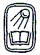
\includegraphics[width=0.07\textwidth]{lt3}
\end{wrapfigure}

\noindent\textit{Издательство«Наука»\\
Главная редакция\\
физико-математической\\
литературы\\}
\newline
\newline
\end{spacing}
\vspace*{-0.7cm}

\begin{wrapfigure}{l}{0.32\textwidth}
\begin{spacing}{0.9}
\noindent Главный редактор\\
\textit{академик} И. К. Кикоин\\
Первый заместитель\\
главного редактора\\
\textit{академик} А.Н. Колмогоров\\
\newline
\textbf{Редакционная коллегия:}\\
М. И. Башмаков,\\
C. Т. Беляев,\\
B. Г. Болтянский,\\
H. Б. Васильев,\\
Ю. Н. Ефремов,\\
B. Г. Зубов,\\
П. Л. Капица,\\
B. А. Кириллин.\\
\textit{главный художник}\\
A. И. Климанов,\\
C. М. Козел.\\
\textit{зам, главного редактора}\\
B. A. Лешковцев,\\
Л. Г. Макар-Лиманов,\\
A. И. Маркушевич,\\
H. А. Патрикеева,\\
И. C. Пстраков,\\
H. X. Розов,\\
A. П. Савин,\\
И. Ш. Слободецкий,\\
\textit{зам, главного редактора}\\
М. Л. Смолянский,\\
Я. А. Смородинский,\\
B. А. Фабрикант,\\
A. Т. Цветков,\\
М. П. Шаскольская,\\
C. И. Шварцбурд,\\
A. И. Ширшов.\\
\newline
\textbf{Редакция:}\\
B. Н. Березин,\\
A. Н. Виленкин,\\
И. Н. Клумова.\\
\textit{художественный редактор}\\
T. М. Макарова,\\
H. А. Минц,\\
Т. С. Петрова,\\
B. А. Тихомирова.\\
\textit{зав. редакцией}\\
Л. В. Чернова\\
\end{spacing}
\end{wrapfigure}

\begin{spacing}{0.5}
\hspace*{-1ex}\textbf{В НОМЕРЕ:}\\
\hspace*{3ex}\rule{9.5cm}{0.4pt}\\
\end{spacing}
\hspace*{-2ex}2 \textit{Н. Я. Виленкин, В. П. Лишевский.} Софья\\
\hspace*{3ex}Васильевна Ковалевская\\
12 \textit{И. И. Воробьев,} Электронный ветер\\
16 \textit{И. Н. Бронштейн.} Гипербола\\
25 \textit{И. П. Стаханов.} Масса и энергия в теории\\
\hspace*{3ex}относительности\\
30 \textit{Л. С. Хренов.} Средства вычислений\\
36 \textit{А. Б. Мигдал.} Письмо школьникам, которые хотят стать\\
\hspace*{3ex}физиками\\
\newline
\hspace*{3ex}\textbf{Математический кружок}\\
39 \textit{3. А. Скопец.} Расстояние между центроидами двух\\
\hspace*{3ex}систем точек\\
\newline
\hspace*{3ex}\textbf{Задачник «Кванта»}\\
44 Победители конкурса «Кванта»\\
46 Задачи М311-M315; ФЗ23 ФЗ27\\
48 Решения задач М273-М279; Ф285-Ф290\\
\newline
\hspace*{3ex}\textbf{Практикум абитуриента}\\
61 \textit{В. К. Егерен, А. Г. Мордкович.} Правильная\\
\hspace*{3ex}пирамида\\
66 \textit{Л. К. Белопухов, М. Г. Сухарев.} Московский институт\\
\hspace*{3ex}нефтехимической и газовой промышленности\\
\newline
69 \textbf{Спрашивайте - отвечаем}\\
\newline
\hspace*{3ex}\textbf{«Квант» для младших школьников}\\
71 Задачи\\
72 \textit{А. П. Савин.} Для чего нужны проценты?\\
\newline
74 \textbf{Ответы, указания, решения} \textit{(3-я стр. обложки)}\\
\newline
\hspace*{3ex}\textbf{Уголок коллекционера}\\
\hspace*{3ex}Смесь (с. 24, 35, 43, 68, 70).
\begin{spacing}{0.7}
\noindent\rule{9.5cm}{0.4pt}\\
\textit{
На первой странице обложки вы видите семейство кривых, координаты (x, y) точек которых удовлетворяют соотношению xy = k при всевозможных k>0. Эти кривые называются гиперболами. Подробнее о гиперболе и ее свойствах вы можете прочесть в статье на с. 16-24.}\\
\rule{9.5cm}{0.4pt}\\
\textit{
\copyright \hspace*{1ex} Главная редакция физико-математической литературы издательства «Наука», «Квант» №3, 1975 год}
\end{spacing}